% begin module reciprocal-function
\begin{frame}
$f(x) = x^{-1} = \frac{1}{x}$ is called the reciprocal function.  Its graph has equation $y = \frac{1}{x}$, or $xy = 1$, and is an hyperbola with the coordinate axes as its asymptotes.
\begin{center}
\psset{xunit=0.6cm, yunit=0.6cm}
\begin{pspicture}(-5, -5)(5,5)
\psframe*[linecolor=white](-5,-5)(5,5)
\psaxes[ticks=none, labels=none]{<->}(0,0)(-5,-5)(5,5)\tiny
%Function formula: (1)/(x)
\rput(1,3){$y=\frac 1 x$}
\psplot[linecolor=red, plotpoints=1000]{0.2}{5}{1 x div } %Function formula: (1)/(x)
\rput(1,3){$y=\frac 1 x$}
\psplot[linecolor=red, plotpoints=1000]{-5}{-0.2}{1 x div }
\fcLabels{4.5}{4.5}
\end{pspicture}
%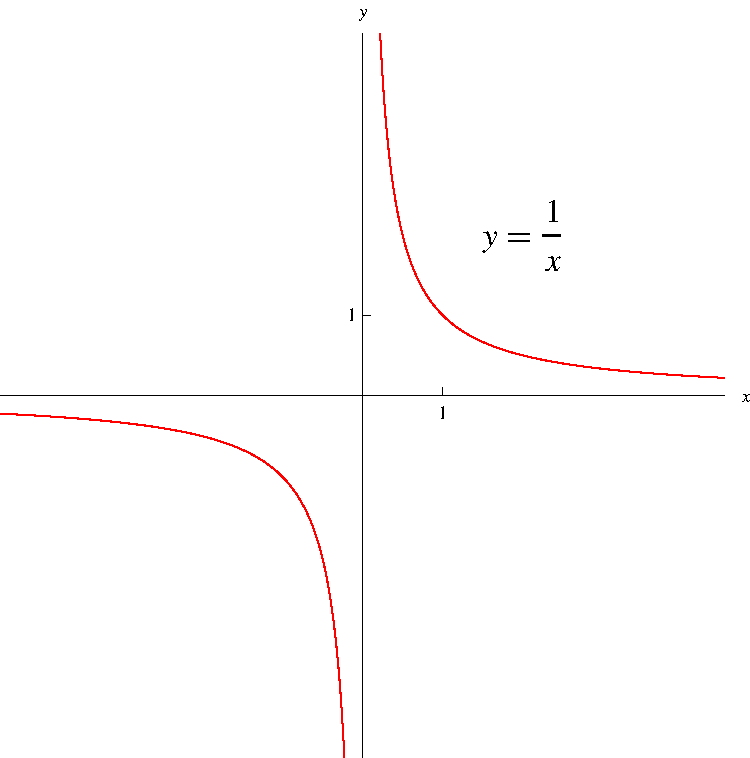
\includegraphics[height=5cm]{precalculus/pictures/reciprocal-function.pdf}%
\end{center}
\end{frame}
% end module reciprocal-function
